% 
% Annual Cognitive Science Conference
% Sample LaTeX Paper -- Proceedings Format
% 
% Original : Ashwin Ram (ashwin@cc.gatech.edu)       04/01/1994
% Modified : Johanna Moore (jmoore@cs.pitt.edu)      03/17/1995
% Modified : David Noelle (noelle@ucsd.edu)          03/15/1996
% Modified : Pat Langley (langley@cs.stanford.edu)   01/26/1997
% Latex2e corrections by Ramin Charles Nakisa        01/28/1997 
% Modified : Tina Eliassi-Rad (eliassi@cs.wisc.edu)  01/31/1998
% Modified : Trisha Yannuzzi (trisha@ircs.upenn.edu) 12/28/1999 (in process)
% Modified : Mary Ellen Foster (M.E.Foster@ed.ac.uk) 12/11/2000
% Modified : Ken Forbus                              01/23/2004
% Modified : Eli M. Silk (esilk@pitt.edu)            05/24/2005
% Modified: Niels Taatgen (taatgen@cmu.edu) 10/24/2006

%% Change ``a4paper'' in the following line to ``letterpaper'' if you are
%% producing a letter-format document.

\documentclass[10pt,letterpaper]{article}

\usepackage{cogsci}
\usepackage{pslatex}
\usepackage{apacite}
\usepackage{graphicx}

\title{One-shot learning of generative speech concepts}
 
\author{Authors}
 
%\author{{\large \bf Morton Ann Gernsbacher (MAG@Macc.Wisc.Edu)} \\
%  Department of Psychology, 1202 W. Johnson Street \\
%  Madison, WI 53706 USA
%  \AND {\large \bf Sharon J. Derry (SDJ@Macc.Wisc.Edu)} \\
%  Department of Educational Psychology, 1025 W. Johnson Street \\
%  Madison, WI 53706 USA}

\begin{document}
\maketitle

\begin{abstract}
\textbf{Keywords:}
speech recognition; category learning; one-shot learning; exemplar generation
\end{abstract}

\section{Introduction}
There has been recent interest in one-shot learning -- the human ability to learn a new concept from just one or a few examples \cite<e.g.,>{CareyBartlett1978,Markman1989,Ahn1992,Xu2007}. Although one-shot learning is an important aspect of everyday cognition, traditional learning algorithms can require tens, hundreds, or thousands of examples before reaching a high level of classification performance. This mismatch poses a challenge to computational approaches for understanding human-level concept learning, yet over the last several decades, the fields of cognitive science and machine learning have made significant progress. Cognitive models have sought to quantitatively explain the way people generalize form just just a few examples in a low-dimensional space \cite{Shepard1987,Feldman1997,Tenenbaum2001}. Other cognitive models and computer vision algorithms become better one-shot learners through ``transfer learning'' or ``learning to learn,'' where previous experience with related concepts helps to inform which dimensions or features are most important for generalization \cite{Bart2005,Colunga2005,FeiFeiFergus2006,KempPerfors2007}.

Despite real progress spanning multiple disciplines, we are still far from a satisfying computational account of one-shot learning. Previous models have been limited by the simplicity of the representations that they learn -- usually prototypes or exemplars in a feature space -- which lack the power necessary for capturing many types of natural concepts \cite{Murphy1985}. While these feature-based approaches can be useful for classification, they provide less insight into how background knowledge interacts with learning or how people generalize in other ways beyond classification, including exemplar generation \cite{Jern2013}, causal inference \cite{Rehder2003}, explanation \cite{Williams2010}, and conceptual combination \cite{Murphy1988}. Given that people learn very rich concepts, even from just one or a few examples, the central computational challenge is to explain how people extract so much information from such limited data.

Analysis-by-synthesis is the classic idea, beginning with Helmholtz, that sensory data can be more richly represented by modeling the causal process that generates it. While these models have been very influential, especially in visual  \cite{Yuille2006} and speech perception \cite{Liberman1967}, there are reasons to believe that this would not be a viable computational strategy for one-shot learning. 


 there are reasons to be skeptical that analysis-by-synthesis could be a plausible computational strategy for one-shot learning. 


 for inferring richer representations for sensory data, but it has not traditionally been applied to one-shot learning. Analysis-by-synthesis is the idea, beginning with Helmholtz, that raw data can be explained by modeling the causal process that generates it. This approach has been most influential in perception, including vision \cite{Yuille2006} and speech \cite{Liberman1967}, where object/stimulus classification involves solving an inverse problem. This inverse problem involves inference rather than learning, since an already acquired generative category model attempts to represent the raw data by producing it. But learning causal process models from data is often difficult and attempted only with many training examples \cite<e.g.,>{HintonNair2006}, and thus there area reasons to be skeptical that analysis-by-synthesis could be a plausible computational strategy for one-shot learning. Given that more complex models require more data for learning \cite<e.g.,>{Geman1992}, how could a generative causal model, rich enough to generate all members of a target class, be learned from just a single example? 

\begin{figure*}[t]
\centering
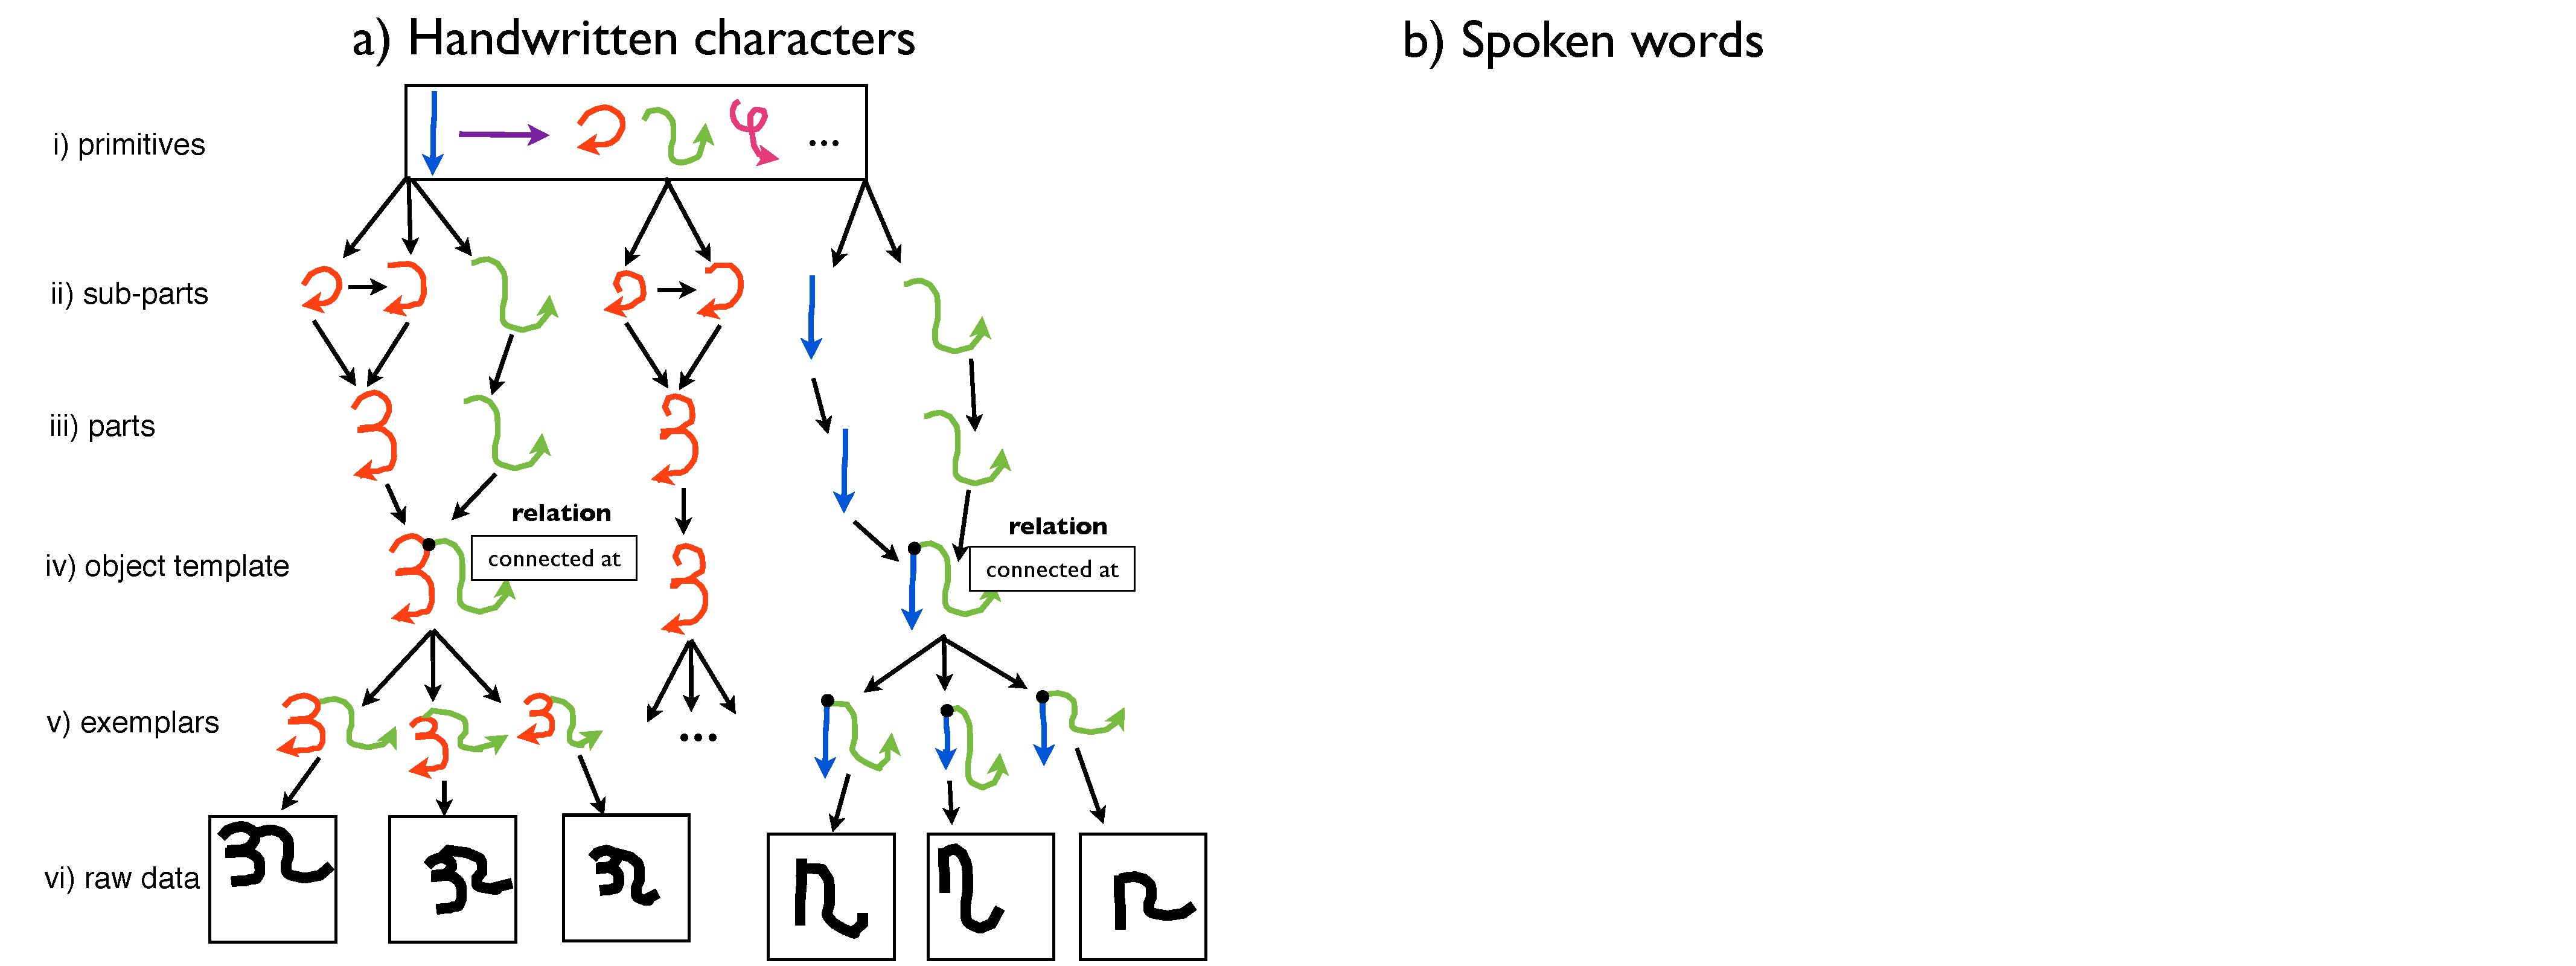
\includegraphics[width=7in]{model.pdf}
\caption{Hierarchical Bayesian modeling as applied to handwritten characters and speech.}
\label{models}
\end{figure*}

One idea is to use a Hierarchical Bayesian model \cite{Gelman2004} to define a ``generative model for generative models,'' with a prior distribution over the space of possible causal processes. This could not lead to effective one-shot learning over causal processes in general, but it could work for a subset of simple processes where fast recovery might be possible. For instance, if a human or machine was trying to learn what a ``tree'' was from just a single example, it would be hopeless to try to represent it by a fully-detailed process of biological growth of trees from tree DNA. But at the right level of abstraction, a tree's essence could be captured by a stochastic program that starts with a single branch and then recursively splits its branches until it terminates.

Despite the inherent challenges in learning generative models from a limited number of examples, recent behavioral and computational work has suggested that this type of learning is well-suited for domains where where the hypothesis space of causal processes can be represented \emph{compositionally} \cite{Lake2012,Lake2013}. [Reference Biederman, free combination of primitives, -- compositionality is an old idea too...] These ideas were applied to the one-shot learning of handwritten characters \cite{Lake2013}, such as letters from a foreign alphabets. Given a raw image of a new character, a Hierarchical Bayesian model learns to represent it by a latent causal process based on a sequence of pen strokes and their spatial relations (Fig. \ref{models}a). Stochastic motor primitives (Fig. \ref{models}a-i) are shared across characters and combined in new ways to make new characters (Fig. \ref{models}a-iv). Thus, the prior distribution on causal models is itself learned from related characters, instantiating another level of model hierarchy and providing a mechanism for transfer learning. Since each inferred character representation is itself generative -- a stochastic motor program -- it can be used to both classify new examples or generate new examples (Fig. \ref{models}a-v) from just a single image of a new character \cite{Lake2013}.

How general is this approach, and can it be applied in non-visual learning? In this paper, we extend these ideas to the one-shot learning of new spoken words, such as a young child learning to recognize and pronounce a new word (the speech sound for ``elephant') or an adult learning a word in a foreign language. This seems to be a promising domain for our general approach, since analysis-by-synthesis has been influential in speech recognition for decades \cite{Halle1962,Liberman1967} and there is a clear compositional structure of phonemes that could be exploited for learning. From the raw speech signal of a word, our model infers a causal representation based on a sequence of phone-like units (Fig. \ref{models}b). Like the characters, the prior distribution on these sequences are learned from experience with other words and can be combined together in new ways to define a new word (Fig. \ref{models}b-iv). Since each inferred word representation is itself generative, it can be used to both classify new examples or generate new examples (Fig. \ref{models}a-v) from just a single instance of a new word. By transferring a prior on sub-unit sequences learned from a corpus of Japanese speech, the model can classify new Japanese words at a level of accuracy similar to English-speaking humans. We also compare humans and the model on another natural form of generalization -- an exemplar generation task.

\section{Model}

\section{Experiment 1: Classification}

One-shot classification (20-way) using Japanese words. Here are factors we are going to manipulate:
\begin{itemize}

\item Classifiers
\begin{itemize}
	\item People (Turkers in the USA, speak no Japanese)
	\item Hierarchical Bayesian (HB) model (trained on English datasets)
	\item HB model (trained on Japanese, using the same corpus and speakers)
	\item Dynamic Time Warp (DTW)
\end{itemize}

\item Stimuli
\begin{itemize}
	\item same gender (training vs. test examples)
	\item different genders
\end{itemize}

\end{itemize}

\subsection{Humans}
Participants in the USA were recruited on Amazon's Mechanical Turk to judge their ability to classify new Japanese words. Participants were shown a sequence of displays, each with a button labeled ``target word'' at the top. Below it there was a grid of buttons numbered ``1'' through ``20,'' each with an associated radio button for response selection (and a general ``submit'' button to complete the trial). Participants were told that each button played a sound clip of a Japanese word, and their job was to pick the sound clip that produces the same word as the target word. Sound clips could be played more than once, and responses were not accepted unless both the target word and the chosen clip were played at least once. 
\subsection{Models}
\subsection{Results}

\section{Experiment 2: Generation}

\subsection{Experiment A: Samples from people} 
Ask people on Turk to generate new examples of Japanese words

\subsection{Experiment B: Evaluation}
 
\begin{itemize}
\item Speech example generators
\begin{itemize}
	\item People (Turkers in the USA, speak no Japanese)
	\item People but reconstructed from MFCCs
	\item Hierarchical Bayesian (HB) model (trained on English datasets)
	\item HB model (trained on Japanese, using the same corpus and speakers)
\end{itemize}
\end{itemize}

\subsection{Experiment C}
Probe model representation by changing phone units

\section{Discussion}

\bibliographystyle{apacite}
\setlength{\bibleftmargin}{.125in}
\setlength{\bibindent}{-\bibleftmargin}

\bibliography{library}
\end{document}

%Categorization is a central problem in several fields, including psychology, machine learning, and AI. Traditional computational approaches to categorization have used sets of exemplars, features, or rules to help discriminate members from non-members, but learning these classic forms of representation typically requires tens, hundreds, or thousands of examples to reach good performance. On the other hand, people can often learn a new category from just one or few examples, an ability often called one-shot learning \cite<e.g.,>{CareyBartlett1978,Markman1989,Ahn1992,Xu2007}. Previous computational accounts have studied how people \cite{Shepard1987,Tenenbaum2001,Feldman1997,Colunga2005}, and machines \cite{MillerMatsakis2000,Bart2005,FeiFeiFergus2006} might generalize from very sparse data, but these models have dealt with only the most classic and simplest types of category representations -- prototypes or sets of exemplars in feature space.

%Categorization is a central problem for both human and machine learning. Traditional computational approaches, as developed in psychology, machine learning, and AI, represent categories as a set of exemplars, features, or rules that help discriminate members from non-members, and learning these classifiers typically require tens, hundreds, or thousands of examples to reach good performance. In contrast, people can often learn a new category from just one or few examples, an ability often called one-shot learning. Furthermore, while people can generalize in many ways beyond classification, it is unclear how these models could apply to other natural forms of category-based generalization. Recent work has shown how a Hierarchical Bayesian model can successfully learn new handwritten characters from one example, where the raw stimuli are decomposed into primitive elements by modeling their underlying causal process. In this paper, we apply this approach to one-shot learning of new spoken words in a foreign language. By transferring learned primitive structure from a corpus of English speech, the model can classify new Japanese words at a level of accuracy similar to English-speaking humans. We also compare humans and the model on another natural form of generalization -- an exemplar generation task.